\section{Active and Efficient Visual Reasoning}
ViThinker \citep{vithinker} is a vision-centric, rather than medical, methods contribution. It provides a deliberate bridge from clinical alignment to efficient reasoning: if a model can request only the perceptual information needed for a decision, medical systems may eventually apply a similar principle to detailed image inspection. Its experiments do not themselves establish medical transfer. Hanqi Jiang is the corresponding and last author of the ICME 2026 Spotlight work.

\subsection{Dynamic perceptual querying}
Related approaches include Aurora, ICoT, CoVT, and MINT-CoT \citep{bigverdi2025perception,gao2025interleaved,qin2025covt,chen2025mintcot}. Fixed visual inputs may devote the same perceptual budget to easy and difficult questions. ViThinker instead generates decision tokens that synthesize expert-aligned visual features on demand. Its curriculum first distills frozen visual experts and then learns task-driven querying with sparsity penalties. At inference, feature synthesis is internal to the model and does not require external tool calls. This makes the sequence of perceptual requests part of reasoning rather than a fixed preprocessing choice.
Figure~\ref{fig:vithinker_overview} shows the training and inference flow.
\begin{figure}[htbp]\centering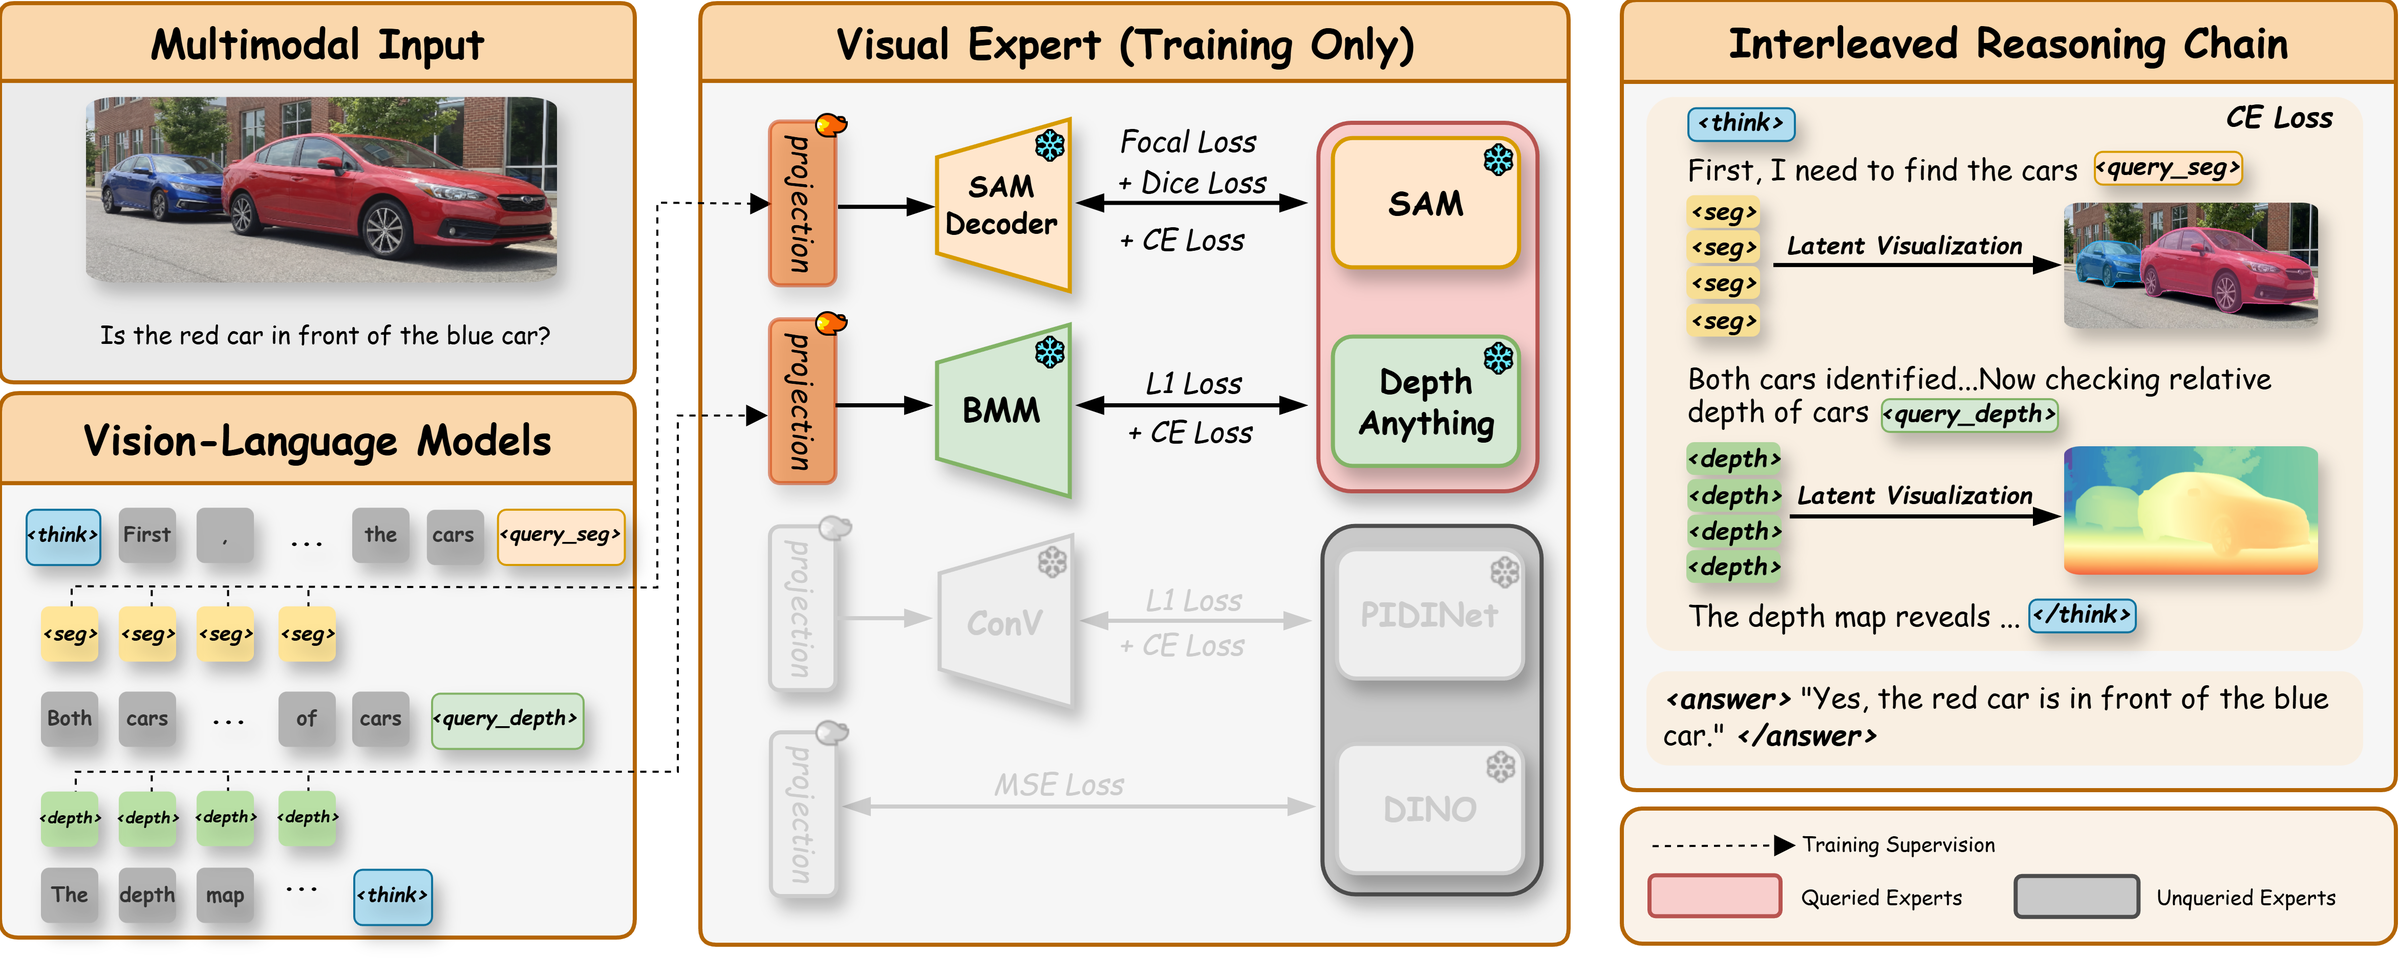
\includegraphics[width=\textwidth,height=.34\textheight,keepaspectratio]{figures/vithinker_overview.png}\caption{For visual question answering, ViThinker processes the image and text into tokens. Its Active Generative Perception Module uses decision tokens to initiate perceptual simulation and reserves observation-token states for expert-aligned features. During training, projection heads align those states with features from frozen vision experts; the curriculum first acquires perceptual skills and then optimizes the querying policy. At inference, generated decision tokens trigger synthesis of expert-aligned features from the model's parameters, without invoking external vision models. Adapted from ViThinker Fig. 1. Source: ViThinker \citep{vithinker}.}\label{fig:vithinker_overview}\end{figure}

The training objective must balance the information gained by additional queries against their cost. A query that never changes the answer wastes budget, but an overly severe sparsity penalty can suppress useful observations. In the reported configuration the sparsity coefficient is $\eta=0.1$, with $N=4$ observation tokens per decision token.

On CV-Bench, ViThinker uses 8.6 tokens versus 16.0 for Full Enumeration, a reduction of 46\%, while matching or exceeding accuracy in the reported comparison. Its average is 70.9\% across seven vision-centric benchmarks, compared with 68.9\% for MINT-CoT; reported individual scores include 81.4 on CV-Bench, 59.1 on BLINK, and 74.2 on RW-QA. The key result is that reduced perceptual use can be measured alongside task performance, rather than inferred from model size alone.

The connection to EDA is conceptual rather than an assertion that the systems share an implementation. EDA selects whether to zoom into an image and then makes its final point available to a declared readout. ViThinker learns internal visual queries. Both ask whether more perception should be acquired when it can change the decision.
